%%%% ijcai17.tex

\typeout{IJCAI-17 Instructions for Authors}

% These are the instructions for authors for IJCAI-17.
% They are the same as the ones for IJCAI-11 with superficical wording
%   changes only.

\documentclass{article}
% The file ijcai17.sty is the style file for IJCAI-17 (same as ijcai07.sty).
\usepackage{ijcai17}

% Use the postscript times font!
\usepackage{times}

% the following package is optional:
%\usepackage{latexsym} 

% Following comment is from ijcai97-submit.tex:
% The preparation of these files was supported by Schlumberger Palo Alto
% Research, AT\&T Bell Laboratories, and Morgan Kaufmann Publishers.
% Shirley Jowell, of Morgan Kaufmann Publishers, and Peter F.
% Patel-Schneider, of AT\&T Bell Laboratories collaborated on their
% preparation.

% These instructions can be modified and used in other conferences as long
% as credit to the authors and supporting agencies is retained, this notice
% is not changed, and further modification or reuse is not restricted.
% Neither Shirley Jowell nor Peter F. Patel-Schneider can be listed as
% contacts for providing assistance without their prior permission.

% To use for other conferences, change references to files and the
% conference appropriate and use other authors, contacts, publishers, and
% organizations.
% Also change the deadline and address for returning papers and the length and
% page charge instructions.
% Put where the files are available in the appropriate places.



\usepackage{times}
\usepackage{epsfig}
\usepackage{graphicx}
\usepackage{amsmath}
\usepackage{amssymb}
\usepackage{subfigure}
\usepackage{scrextend}
\usepackage{enumerate}
\usepackage{overpic}
%\usepackage{multicol}
\usepackage[table]{xcolor}
\newcommand{\row}[2] {#1_{#2 \cdot}}
\newcommand{\col}[2] {#1_{\cdot #2}}

\usepackage[small]{caption}

% Include other packages here, before hyperref.

% If you comment hyperref and then uncomment it, you should delete
% egpaper.aux before re-running latex.  (Or just hit 'q' on the first latex
% run, let it finish, and you should be clear).
\usepackage[breaklinks=true,bookmarks=false]{hyperref}


\begin{document}

%%%%%%%%% TITLE
\title{Demystifying Neural Style Transfer}

%\author{Anonymous Submission}
\author{Yanghao Li$^\dagger$~~~~~ Naiyan Wang$^\ddagger$~~~~~ Jiaying Liu$^\dagger$\thanks{Corresponding author}~~~~~ Xiaodi Hou$^\ddagger$\\
$^\dagger$ Institute of Computer Science and Technology, Peking University~~~~~\\
$^\ddagger$ TuSimple\\
{ lyttonhao@pku.edu.cn}~~{ winsty@gmail.com}~~
{ liujiaying@pku.edu.cn}~~
{ xiaodi.hou@gmail.com}
% {\tt\small \{lyttonhao, liujiaying\}@pku.edu.cn}~~~{\tt\small \{winsty, shijianping5000, xiaodi.hou\}@gmail.com}
}

\maketitle
\rowcolors{2}{white}{gray!25}
%\thispagestyle{empty}

\graphicspath{{figures/}}

%%%%%%%%% ABSTRACT
\begin{abstract}
%Although Deep Convolutional Neural Networks (CNNs) have liberated their power in various computer vision tasks, the most important components of CNN, convolutional layers and fully connected layers, are still limited to linear transformations. In this paper, we propose a novel Factorized Bilinear (FB) layer to model the pairwise feature interactions by considering the quadratic terms in the transformations. Compared with existing methods that tried to incorporate complex non-linearity structures into CNNs, the factorized parameterization makes our FB layer only require a linear increase of parameters and affordable computational cost. To further reduce the risk of overfitting of the FB layer, a specific remedy called DropFactor is devised during the training process. We also analyze the connection between FB layer and some existing models, and show FB layer is a generalization to them. Finally, we validate the effectiveness of FB layer on several widely adopted datasets including CIFAR-10, CIFAR-100 and ImageNet, and demonstrate superior results compared with various state-of-the-art deep models.

Neural Style Transfer~\cite{neuralart} has recently demonstrated very exciting results which catches eyes in both academia and industry. Despite the amazing results, the principle of neural style transfer, especially why the Gram matrices could represent style remains unclear. In this paper, we propose a novel interpretation of neural style transfer by treating it as a domain adaptation problem. Specifically, we theoretically show that matching the Gram matrices of feature maps is equivalent to minimize the Maximum Mean Discrepancy (MMD) with the second order polynomial kernel. Thus, we argue that the essence of neural style transfer is to match the feature distributions between the style images and the generated images. To further support our standpoint, we experiment with several other distribution alignment methods, and achieve appealing results. We believe this novel interpretation connects these two important research fields, and could enlighten future researches.

\end{abstract}

\begin{section}{Introduction}

Transferring the style from one image to another image is an interesting yet difficult problem. There have been many efforts to develop efficient methods for automatic style transfer~\cite{hertzmann2001image,efros2001image,efros1999texture,shih2014style,kwatra2005texture}. Recently, Gatys \emph{et al.} proposed a seminal work~\cite{neuralart}: It captures the style of artistic images and transfer it to other images using Convolutional Neural Networks (CNN). This work formulated the problem as finding an image that matching both the content and style statistics based on the neural activations of each layer in CNN. It achieved impressive results and several follow-up works improved upon this innovative approaches~\cite{johnson2016perceptual,ulyanov2016texture,ruder2016artistic,ledig2016photo}. Despite the fact that this work has drawn lots of attention, the fundamental element of style representation: the Gram matrix in~\cite{neuralart} is not fully explained. The reason why Gram matrix can represent artistic style still remains a mystery.

In this paper, we propose a novel interpretation of neural style transfer by casting it as a special domain adaptation~\cite{beijbom2012domain,patel2015visual} problem. We theoretically prove that matching the Gram matrices of the neural activations can be seen as minimizing a specific Maximum Mean Discrepancy (MMD)~\cite{mmd}. This reveals that neural style transfer is intrinsically a process of distribution alignment of the neural activations between images. Based on this illuminating analysis, we also experiment with other distribution alignment methods, including MMD with different kernels and a simplified moment matching method. These methods achieve diverse but all reasonable style transfer results. Specifically, a transfer method by MMD with linear kernel achieves comparable visual results yet with a lower complexity. Thus, the second order interaction in Gram matrix is not a must for style transfer. Our interpretation provides a promising direction to design style transfer methods with different visual results. To summarize, our contributions are shown as follows:
\begin{enumerate}
\item First, we demonstrate that matching Gram matrices in neural style transfer~\cite{neuralart} can be reformulated as minimizing  MMD with the second order polynomial kernel.
\item Second, we extend the original neural style transfer with different distribution alignment methods based on our novel interpretation.
\end{enumerate}

\end{section}

\section{Related Work and Background}\label{sec:related}
\subsection{The Graphics Processing Unit (GPU)}
The GPU of today is a highly parallel, throughput-focused programmable processor. GPU programs (``kernels'') launch over a \emph{grid} of numerous \emph{blocks}; the GPU hardware maps blocks to available parallel cores. Each block typically consists of dozens to thousands of individual \emph{threads}, which are arranged into 32-wide \emph{warps}. Warps run under SIMD control on the GPU hardware. While blocks cannot directly communicate with each other within a kernel, threads within a block can, via a user-programmable 48~kB \emph{shared-memory}, and threads within a warp additionally have access to numerous warp-wide instructions. The GPU's global memory (DRAM), accessible to all blocks during a computation, achieves its maximum bandwidth only when neighboring threads access neighboring locations in the memory; such accesses are termed \emph{coalesced}.
In this work, when we use the term ``\emph{global}'', we mean an operation of device-wide scope. Our term ``\emph{local}'' refers to an operation limited to smaller scope (e.g., within a thread, a warp, a block, etc.), which we will specify accordingly. The major difference between the two is the cost of communication: global operations must communicate through global DRAM, whereas local operations can communicate through lower-latency, higher-bandwidth mechanisms like shared memory or warp-wide intrinsics.
Lindholm et al.~\shortcite{Lindholm:2008:NTA} and Nickolls et al.~\shortcite{Nickolls:2008:SPP} provide more details on GPU hardware and the GPU programming model, respectively.

We use NVIDIA's CUDA as our programming language in this work~\cite{NVIDIA:2016:CUDA}. CUDA provides several warp-wide voting and shuffling instructions for intra-warp communication of threads. All threads within a warp can see the result of a user-specified predicate in a bitmap variable returned by \texttt{\_\_ballot(predicate)}~\cite[Ch.~B13]{NVIDIA:2016:CUDA}. Any set bit in this bitmap denotes the predicate  being non-zero for the corresponding thread. Each thread can also access registers from other threads in the same warp with \texttt{\_\_shfl(register\_name, source\_thread)}~\cite[Ch.~B14]{NVIDIA:2016:CUDA}. Other shuffling functions such as \texttt{\_\_shfl\_up()} or \texttt{\_\_shfl\_xor()} use relative addresses to specify the source thread.
In CUDA, threads also have access to some efficient integer intrinsics, e.g., \texttt{\texttt{\_\_popc()}} for counting the number of set bits in a register.

\subsection{Parallel primitive background}
In this paper we leverage numerous standard parallel primitives, which we briefly describe here. A \emph{reduction} inputs a vector of elements and applies a binary associative operator (such as addition) to reduce them to a single element; for instance, sum-reduction simply adds up its input vector.
The \emph{scan} operator takes a vector of input elements and an associative binary operator, and returns an output vector of the same size as the input vector.
In exclusive (resp., inclusive) scan, output location $i$ contains the reduction of input elements 0 to $i-1$ (resp., 0 to $i$).
Scan operations with binary addition as their operator are also known as \emph{prefix-sum}~\cite{Harris:2007:PPS:nourl}.
Any reference to a multi- operator (multi-reduction, multi-scan) refers to running multiple instances of that operator in parallel on separate inputs. \emph{Compaction} is an operation that filters a subset of its input elements into a smaller output array while preserving the order.

\subsection{Multisplit and Histograms}
Many multisplit implementations, including ours, depend heavily on knowledge of the total number of elements within each bucket (bin), i.e., histogram computation.
Previous competitive GPU histogram implementations share a common philosophy: divide the problem into several smaller sized subproblems and assign each subproblem to a thread, where each thread sequentially processes its subproblem and keeps track of its own \emph{privatized} local histogram.
Later, the local histograms are aggregated to produce a globally correct histogram.
There are two common approaches to this aggregation: 1) using atomic operations to correctly add bin counts together (e.g., Shams and Kennedy~\shortcite{Shams:2007:EHA}), 2)~storing per-thread sequential histogram computations and combining them via a global reduction (e.g., Nugteren et al.~\shortcite{Nugteren:2011:HPP}).
The former is suitable when the number of buckets is large; otherwise atomic contention is the bottleneck.
The latter avoids such conflicts by using more memory (assigning exclusive memory units per-bucket and per-thread), then performing device-wide reductions to compute the global histogram.

The hierarchical memory structure of NVIDIA GPUs, as well as NVIDIA's more recent addition of faster but local shared memory atomics (among all threads within a thread block), provides more design options to the programmer.
With these features, the aggregation stage could be performed in multiple rounds from thread-level to block-level and then to device-level (global) results.
Brown et al.~\shortcite{Brown:2012:MFH} implemented both Shams's and Nugteren's 
aforementioned methods, as well as a variation of their own, focusing only on 8-bit data, considering careful optimizations that make the best use of the GPU, including loop unrolling, thread coarsening, and subword parallelism, as well as others.
Recently, NVIDIA's CUDA Unbound (CUB)~\cite{Merrill:2015:CUB} library has included an efficient and consistent histogram implementation that carefully uses a minimum number of shared-memory atomics to combine per-thread privatized histograms per thread-block, followed by aggregation via global atomics. CUB's histogram supports any data type (including multi-channel 8-bit inputs) with any number of bins.

Only a handful of papers have explored multisplit as a standalone primitive. He et al.~\cite{He:2008:RJG} implemented multisplit by reading multiple elements with each thread, sequentially computing their histogram and local offsets (their order among all elements within the same bucket and processed by the same thread), then storing all results (histograms and local offsets) into memory. Next, they performed a device-wide scan operation over these histogram results and scattered each item into its final position. Their main bottlenecks were the limited size of shared memory, an expensive global scan operation, and random non-coalesced memory accesses.%
\footnote{On an NVIDIA 8800 GTX GPU, for 64 buckets, He et al.\ reported 134~Mkeys/sec. As a very rough comparison, our GeForce GTX 1080 GPU has 3.7x the memory bandwidth, and our best 64-bucket implementation runs 126 times faster.}

Patidar~\cite{Patidar:2009:SPD} proposed two methods with a particular focus on a large number of buckets (more than 4k): one based on heavy usage of shared-memory atomic operations (to compute block level histogram and intra-bucket orders), and the other by iterative usage of basic binary split for each bucket (or groups of buckets). Patidar used a combination of these methods in a hierarchical way to get his best results.%
\footnote{On an NVIDIA GTX280 GPU, for 32 buckets, Patidar reported 762~Mkeys/sec. As a very rough comparison, our GeForce GTX 1080 GPU has 2.25x the memory bandwidth, and our best 32-bucket implementation runs 23.5 times faster.}
Both of these multisplit papers focus only on key-only scenarios, while data movements and privatization of local memory become more challenging with key-value pairs.


% \begin{section}{Background}
In this section, we briefly review the original neural style transfer~\cite{neuralart} and the Maxmimum Mean Discrepancy (MMD)~\cite{mmd} which is closely related to our work.
\begin{paragraph}{Neural Style Transfer}
\end{paragraph}

\begin{paragraph}{Maxmimum Mean Discrepancy}
\end{paragraph}
\end{section}

\begin{section}{Understanding Neural Style Transfer}
In this section, we first theoretically demonstrate that matching Gram matrices is equivalent to minimizing a specific form of MMD. Then based on this interpretation, we extend the original neural style transfer with different distribution alignment methods.

Before explaining our observation, we first briefly review the original neural style transfer approach~\cite{neuralart}. The goal of style transfer is to generate a stylized image $\mathbf{x}^*$ given a content image $\mathbf{x}_c$ and a reference style image $\mathbf{x}_s$. The feature maps of $\mathbf{x}^*$, $\mathbf{x}_c$ and $\mathbf{x}_s$ in the layer $l$ of a CNN are denoted by $\mathbf{F}^l \in \mathbb{R}^{N_l \times M_l}$, $\mathbf{P}^l \in \mathbb{R}^{N_l \times M_l}$ and $\mathbf{S}^l \in \mathbb{R}^{N_l \times M_l}$ respectively, where $N_l$ is the number of the feature maps in the layer $l$ and $M_l$ is the height times the width of the feature map.

In \cite{neuralart}, neural style transfer iteratively generates $\mathbf{x}^*$ by optimizing a content loss and a style loss:
\begin{equation}\label{eq:total_loss}
\begin{aligned}
\mathcal{L} = \alpha\mathcal{L}_{content} + \beta\mathcal{L}_{style},
\end{aligned}
\end{equation}
where $\alpha$ and $\beta$ are the weights for content and style losses, $\mathcal{L}_{content}$ is defined by the squared error between the feature maps of a specific layer $l$ for $\mathbf{x}^*$ and $\mathbf{x}_c$:
\begin{equation}
\begin{aligned}
\mathcal{L}_{content} = \frac{1}{2}\sum_{i=1}^{N_l}\sum_{j=1}^{M_l}(F_{ij}^l - P_{ij}^l)^2,
\end{aligned}
\end{equation}
and $\mathcal{L}_{style}$ is the sum of several style loss $\mathcal{L}_{style}^{l}$ in different layers:
\begin{equation}
\begin{aligned}
\mathcal{L}_{style} = \sum_{l} w_l\mathcal{L}_{style}^{l},
\end{aligned}
\end{equation}
where $w_l$ is the weight of the loss in the layer $l$ and  $\mathcal{L}_{style}^{l}$ is defined by the squared error between the features correlations expressed by Gram matrices of $\mathbf{x}^*$ and $\mathbf{x}_s$:
\begin{equation}\label{eq_style}
\begin{aligned}
\mathcal{L}_{style}^l = \frac{1}{4N_l^2M_l^2}\sum_{i=1}^{N_l}\sum_{j=1}^{N_l}(G_{ij}^l - A_{ij}^l)^2,
\end{aligned}
\end{equation}
where the Gram matrix $\mathbf{G}^l \in \mathbb{R}^{N_l \times N_l}$ is the inner product between the vectorized feature maps of $\mathbf{x}^*$ in layer $l$:
\begin{equation}
\begin{aligned}
G_{ij}^l = \sum_{k=1}^{M_l}F_{ik}^lF_{jk}^l,
\end{aligned}
\end{equation}
and similarly $\mathbf{A}^l$ is the Gram matrix corresponding to $\mathbf{S}^l$.

\begin{figure*}[hbtp]
\begin{footnotesize}
\begin{equation}\label{eq:provemmd}
\begin{aligned}
&\mathcal{L}_{style}^l = \frac{1}{4N_l^2M_l^2}\sum_{i=1}^{N_l}\sum_{j=1}^{N_l}(\sum_{k=1}^{M_l}F_{ik}^lF_{jk}^l - \sum_{k=1}^{M_l}S_{ik}^lS_{jk}^l)^2\\
&=  \frac{1}{4N_l^2M_l^2}\sum_{i=1}^{N_l}\sum_{j=1}^{N_l}\Big( 
		(\sum_{k=1}^{M_l}F_{ik}^lF_{jk}^l)^2 +
		(\sum_{k=1}^{M_l}S_{ik}^lS_{jk}^l)^2 -
		2(\sum_{k=1}^{M_l}F_{ik}^lF_{jk}^l)(\sum_{k=1}^{M_l}S_{ik}^lS_{jk}^l) \Big)\\
&=  \frac{1}{4N_l^2M_l^2}\sum_{i=1}^{N_l}\sum_{j=1}^{N_l}\sum_{k_1=1}^{M_l}\sum_{k_2=1}^{M_l} ( F_{ik_1}^l F_{jk_1}^l F_{ik_2}^l F_{jk_2}^l + 
S_{ik_1}^l S_{jk_1}^l S_{ik_2}^l S_{jk_2}^l - 2 F_{ik_1}^l F_{jk_1}^l  S_{ik_2}^l S_{jk_2}^l)\\
&= \frac{1}{4N_l^2M_l^2}\sum_{k_1=1}^{M_l}\sum_{k_2=1}^{M_l} \sum_{i=1}^{N_l}\sum_{j=1}^{N_l} ( F_{ik_1}^l F_{jk_1}^l F_{ik_2}^l F_{jk_2}^l + 
S_{ik_1}^l S_{jk_1}^l S_{ik_2}^l S_{jk_2}^l - 2 F_{ik_1}^l F_{jk_1}^l  S_{ik_2}^l S_{jk_2}^l)\\
&= \frac{1}{4N_l^2M_l^2}\sum_{k_1=1}^{M_l}\sum_{k_2=1}^{M_l} 
   \Big( (\sum_{i=1}^{N_l}F_{ik_1}^lF_{ik_2}^l)^2 + 
         (\sum_{i=1}^{N_l}S_{ik_1}^lS_{ik_2}^l)^2 - 
         2(\sum_{i=1}^{N_l}F_{ik_1}^lS_{ik_2}^l)^2
   \Big)\\
&= \frac{1}{4N_l^2M_l^2}\sum_{k_1=1}^{M_l} \sum_{k_2=1}^{M_l} 
   \Big(  ({\col{\mathbf{f}^l}{k_1}}^T \col{\mathbf{f}^l}{k_2} )^2  + 
   		  ({\col{\mathbf{s}^l}{k_1}}^T \col{\mathbf{s}^l}{k_2} )^2  -
   		  2 ({\col{\mathbf{f}^l}{k_1}}^T \col{\mathbf{s}^l}{k_2} )^2 
   \Big),
\end{aligned}
\end{equation}
\end{footnotesize}
\vspace{-2mm}
\end{figure*}

\begin{subsection}{Reformulation of the Style Loss}
In this section, we reformulated the style loss $\mathcal{L}_{style}$ in Eq.~\ref{eq_style}. By expanding the Gram matrix in Eq.~\ref{eq_style}, we can get the formulation of Eq.~\ref{eq:provemmd}, where $\col{\mathbf{f}^l}{k}$ and $\col{\mathbf{s}^l}{k}$ is the $k$-th column of $\mathbf{F}^l$ and $\mathbf{S}^l$.

By using the second order degree polynomial kernel $k(\mathbf{x}, \mathbf{y}) = (\mathbf{x}^T\mathbf{y})^2$, Eq.~\ref{eq:provemmd} can be represented as:
\begin{equation}\label{eq:prove_result}
\begin{aligned}
\mathcal{L}_{style}^l =& \frac{1}{4N_l^2M_l^2}\sum_{k_1=1}^{M_l}\sum_{k_2=1}^{M_l}  
	\Big( k(\col{\mathbf{f}^l}{k_1}, \col{\mathbf{f}^l}{k_2}) \\
		 & + k(\col{\mathbf{s}^l}{k_1}, \col{\mathbf{s}^l}{k_2}) 
		 - 2k(\col{\mathbf{f}^l}{k_1}, \col{\mathbf{s}^l}{k_2})
	\Big)\\
	=& \frac{1}{4N_l^2} \text{MMD}^2[\mathcal{F}^{l}, \mathcal{S}^{l}],
\end{aligned}
\end{equation}
where $\mathcal{F}^{l}$ is the feature set of $\mathbf{x}^*$ where each sample is a column of $\mathbf{F}^l$, and $\mathcal{S}^{l}$ corresponds to the style image $\mathbf{x}_s$. In this way, the activations at each position of feature maps is considered as an individual sample. Consequently, the style loss ignores the positions of the features, which is desired for style transfer. In conclusion, the above reformulations suggest two important findings:
\begin{enumerate}
\item The style of a image can be intrinsically represented by feature distributions in different layers of a CNN.
\item The style transfer can be seen as a distribution alignment process from the content image to the style image. 
\end{enumerate}
\end{subsection}

\begin{subsection}{Different Adaptation Methods for Neural Style Transfer}\label{sec:methods}
Our interpretation reveals that neural style transfer can be seen as a problem of distribution alignment, which is also at the core in domain adaptation. If we consider the style of one image in a certain layer of CNN as a ``domain'', style transfer can also be seen as a special domain adaptation problem. The specialty of this problem lies in that we treat the feature at each position of feature map as one individual data sample, instead of that in traditional domain adaptation problem in which we treat each image as one data sample. (\emph{e.g.} The feature map of the last convolutional layer in VGG-19 model is of size $14 \times 14$, then we have totally 196 samples in this ``domain''.)

%The difference between the distribution alignment in these two problems is that the sample in neural style transfer is position-level (a feature vector in one position of a feature map for one image), while the sample in domain adaptation is image-level (a feature vector for a single image). 

Inspired by the studies of domain adaptation, we extend neural style transfer with different adaptation methods in this subsection.

\begin{paragraph}{MMD with Different Kernel Functions}
As shown in Eq.~\ref{eq:prove_result}, matching Gram matrices in neural style transfer can been seen as a MMD process with second order polynomial kernel. It is very natural to apply other kernel functions for MMD in style transfer. First, if using MMD statistics to measure the style discrepancy, the style loss can be defined as:
\begin{equation}\label{eq:style_mmd}
\begin{aligned}
&\mathcal{L}_{style}^l = \frac{1}{Z^l_k}\text{MMD}^2[\mathcal{F}^{l}, \mathcal{S}^{l}],\\
	&= \frac{1}{Z^l_k}\sum_{i=1}^{M_l}\sum_{j=1}^{M_l}\Big( 
		k(\col{\mathbf{f}^l}{i}, \col{\mathbf{f}^l}{j}) +
		  k(\col{\mathbf{s}^l}{i}, \col{\mathbf{s}^l}{j}) - 2k(\col{\mathbf{f}^l}{i}, \col{\mathbf{s}^l}{j})
	\Big),
\end{aligned}
\end{equation}
where $Z^l_k$ is the normalization term corresponding to different scale of the feature map in the layer $l$ and the choice of  kernel function. Theoretically, different kernel function implicitly maps features to different higher dimensional space. Thus, we believe that different kernel functions should capture different aspects of a style. We adopt the following three popular kernel functions in our experiments:
\begin{enumerate}[{(1)}]
	\item Linear kernel: $k(\mathbf{x}, \mathbf{y}) = \mathbf{x}^T\mathbf{y}$;
	\item Polynomial kernel: $k(\mathbf{x}, \mathbf{y}) = (\mathbf{x}^T\mathbf{y} + c)^d$;
	\item Gaussian kernel: $k(\mathbf{x}, \mathbf{y}) = \exp\big( -\frac{\|\mathbf{x} - \mathbf{y}\|_2^2}{2\sigma^2}  \big)$.
\end{enumerate}
For polynomial kernel, we only use the version with $d = 2$. Note that matching Gram matrices is equivalent to the polynomial kernel with $c = 0$ and $d = 2$. For the Gaussian kernel, we adopt the unbiased estimation of MMD~\cite{gretton2012optimal}, which samples $M_l$ pairs in Eq.~\ref{eq:style_mmd} and thus can be computed with linear complexity. % Using the MMD statistics the style loss , the style loss Eq.~\ref{eq:prove_result} can be changed to  different forms:
% \begin{equation}
% \begin{aligned}
% \mathcal{L}_{style}^l = \left\{
% 		\begin{array}{ll}
% 			\frac{1}{N_lM_l}\sum_{i,j=1}^{M_l} 
% 	\Big( {\col{\mathbf{F}^l}{i}}^T \col{\mathbf{F}^l}{j} +
% 		  {\col{\mathbf{S}^l}{i}}^T \col{\mathbf{S}^l}{j} + 
% 		  -2{\col{\mathbf{F}^l}{i}}^T \col{\mathbf{S}^l}{j} \Big)\\
% 			y\\
% 		\end{array}
% \right.
% \end{aligned}
% \end{equation}


\end{paragraph}

\begin{paragraph}{BN Statistics Matching} In~\cite{adabn}, the authors found that the statistics (\emph{i.e.} mean and variance) of Batch Normalization (BN) layers contains the traits of different domains. Inspired by this observation, they utilized separate BN statistics for different domain. This simple operation aligns the different domain distributions effectively. As a special domain adaptation problem, we believe that BN statistics of a certain layer can also represent the style. Thus, we construct another style loss by aligning the BN statistics (mean and standard deviation) of two feature maps between two images:
\begin{equation}
%\begin{small}
\begin{aligned}
&\mathcal{L}_{style}^l = \frac{1}{N_l} \sum_{i=1}^{N_l}\Big( ( \mu^i_{F^l} - \mu^i_{S^l} )^2 + ( \sigma^i_{F^l} - \sigma^i_{S^l} )^2 \Big),
\end{aligned}
%\end{small}
\end{equation}
where $\mu^i_{F^l}$ and $\sigma^i_{F^l}$ is the mean and standard deviation of the $i$-th feature channel among all the positions of the feature map in the layer $l$ for image $\mathbf{x}^*$:
\begin{equation}
%\begin{small}
\begin{aligned}
\mu^i_{F^l} = \frac{1}{M_l} \sum_{j=1}^{M_l} F^l_{ij}, \quad
{\sigma^i_{F^l}}^2 =  \frac{1}{M_l} \sum_{j=1}^{M_l} (F^l_{ij} - \mu^i_{F^l})^2,
\end{aligned}
%\end{small}
\end{equation}
and $\mu^i_{S^l}$ and $\sigma^i_{S^l}$ correspond to the style image $\mathbf{x}_s$.
\end{paragraph}


The aforementioned style loss functions are all differentiable and thus the style matching problem can be solved by back propagation iteratively.
\end{subsection}

\end{section}



% \input{src/relation.tex}

% !TEX root = ../EDBT.tex
\begin{figure}
\centering
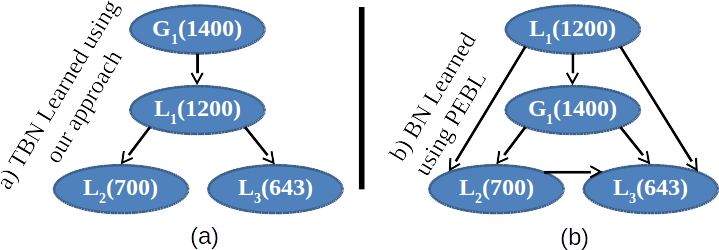
\includegraphics[width = 100mm]{Figures/g1Network.png}
\vspace{6pt}
\caption{Structure learned of $G_1$ using two different approaches}
\label{fig:g1net}
%\vspace{-10pt}
\end{figure}

We present the accuracy of our predictions on a real-life dataset from a global market research organization. We set a threshold $\tau$ on CoP, and predictions with a CoP $< \tau$ are routed for human annotation. We also measure the accuracies of our predictions for different values of $\tau$.

\textit{\textbf{Data description}}: We have data for carbonated drinks of $26$K unique products from a single geography, contained in two datasets:
a)~\textbf{Local DB}: It contains 26K products with each product having $49$ local characteristics, where cardinality of local characteristics varies from tens to thousands. It also contains descriptions of products given by retailers of that product, where number of descriptions of a single product varies from tens to hundreds. b)~\textbf{Global DB}: It contains four global characteristics with cardinality varying from tens to thousands.

\textbf{\textit{Data Preparation:}} We predict four global characteristics $G_1$, $G_2$, $G_3$, and $G_4$ for two cases, with varying ratio of split between training, validation and test datasets. \textbf{\textit{Case-1}}(60:20:20) has 60\% training, 20\% validation and 20\% test and \textbf{\textit{Case-2}} has this ratio as 20:20:60. \textbf{NOTE:} While Case-1 uses a traditional split of training vs testing data, Case-2 is more realistic, since in practice preparing a training data by manual data labeling is costly: For example, we would like to `onboard' a data from a particular dataset 
by manually annotating only a small fraction (e.g. 20\%) of records and automate the remainder or we might like to board 
data from one organization (e.g. retailer or distributor) in a particular geography in the hope that data from remaining sources in that
geography share similar local characteristics, eliminating manual annotation for a large volume of data. 
To simulate this practical scenario, we used the first few records from the local dataset, which happened to contain only 10\% or so of the
total possible values of each global attribute.

For SBM, $\eta$ relevant local characteristics was chosen for every $G_j$. Figure~\ref{fig:g1net}, compares the Bayesian network structure learned using our approach and another learned using an open source python library Pebl \cite{shah2009python}, for the global characteristic $G_1$. Clearly, network obtained using Pebl (Figure~\ref{fig:g1net}(b)) is more complex as compared to ours \ref{fig:g1net}(a), as the size of CPTs of these are of the order of a)~$1200\times1400$ and b)~$1200\times1400\times700\times643$ respectively. %Scaling factor $\lambda=0.1$ was used in Equation~\ref{eq:soft} for predictions using UTS model.

\begin{figure}
\centering
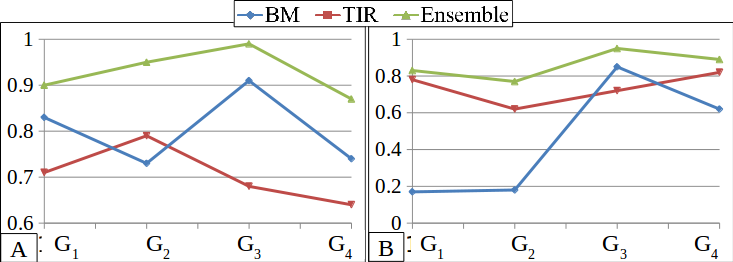
\includegraphics[width= 90mm]{Figures/Case1-2.png}
%\vspace{-10pt}
\caption{x-axis: global characteristics, y-axis: A)~Predictive accuracy for Case-1, B)~Predictive accuracy for Case-2}
%\vspace{-8pt}
\label{fig:case-1}
%\vspace{-8pt}
\end{figure}

Figure \ref{fig:case-1}, shows the prediction accuracy of four global characteristic for Case-1 and Case-2 respectively. Here, the accuracy is a ratio of correctly predicted products to the total number of products. In Case-1, accuracy of Ensemble model is in the range of 85 to 99\%  and it outperforms both SBM and UTS for all four global characteristics.

\textbf{\textit{Baseline Comparison}}: We also compared our approach with record matching method implemented in a framework called FEBRL\cite{christen2008febrl}. For attribute matching, we tried three similarity measures winkler, tokenset, trigam and show the results with winkler which outperforms the rest. We tested this approach for the Case-1 on the smaller dataset (5K products). Table~\ref{table:comparison}, shows the comparison of the prediction accuracy of four global attributes using our Ensemble approach and FEBRL. This suggests that our approach outperforms and also shows that accuracy of FEBRL decreases for high cardinality global attributes. FEBRL did not work on, 26k products, on a machine with 16GB RAM, Intel Core i7-3520M CPU 2.90GHz* 4, 64 bit. We did not try the blocking method as main motive of our problem is to improve accuracy of prediction, and not the time complexity. 
\renewcommand{\arraystretch}{}
\begin{table}
%\scriptsize 
  \centering
  %\small
  \begin{tabular}{|c|c|c|c|} 
   \hline
   Global att. & Num of states & FEBRL(winkler) & Ensemble \\
   \hline
   $G_1$ & 107 & 86\% & 93\% \\
   \hline
   $G_2$ & 154 & 57\% & 95.2\% \\
   \hline
   $G_3$ & 3 & 99.3\% & 99.2\% \\
   \hline
   $G_4$ & 13 & 95.4\% & 99.4\% \\
   \hline 
  \end{tabular}
  %\vspace{4pt}
\caption{Comparison of our approach with FEBRL}
  \label{table:comparison}
  %\vspace{-15pt}
\end{table}
\textbf{Case-2} (Figure \ref{fig:case-1}-B), naturally renders the SBM less accurate, since the training data contains only 10\% of possible states of each global characteristic. However, it is compensated by the performance of UTS, which searches the target set of global attribute values from the
retailer descriptions. Combining these models using our Ensemble model the accuracy of four global characteristics reaches 78 to 93\%.

\textbf{\textit{CoP Threshold for human annotation:}} We define three categories: a)~\textbf{P-C:} Number of products \textit{predicted correctly} by our approach for which CoP $> \tau$. b)~\textbf{P-I:} Number of products \textit{predicted incorrectly}, for which CoP $> \tau$. c)~ \textbf{NP:} Products which we choose \textit{not to predict}, i.e., products with CoP $\leq \tau$. We select $\tau$ in order to maximize P-C and minimize P-I category, while not increasing NP so much that exercise becomes almost entirely manual. Since products in the P-I category are more costly for a company as compared to NP category, we give more weight to P-I while learning $\tau$. Table~\ref{table:categories}, shows the percentage of products in each category (P-C, P-I, NP) on validation set along with the threshold $\tau$ values for both cases. It shows that for given $\tau$, percentage of products in P-C category is in the range of 81-96\% for Case-1, whereas, it ranges from 70 to 96\% for Case-2. Also, the average percentage of products in P-I category is only around 5\%. These numbers establish that CoP is a good measure for reliability of predictions. Figure~\ref{fig:PC-2}, shows the variation in the percentage of products in test set of each category with respect to threshold value $\tau$ for both Case-1 and Case-2, for the global characteristic $G_1$. It validates the optimal values of $\tau$ learned using validation set, 0.5 for Case-1 and 0.6 for Case-2.

The process of aggregate analysis, comparing global market share and sales of product categories is carried out in our platform \textbf{\textit{iFuse}}\cite{singh2016visual} (Figure~\ref{fig:iFuse}). Figure~\ref{fig:iFuse}(a),(b) shows the data tile and cart view of iFuse representing the attributes of the local DB and global DB to be linked together. Figure~\ref{fig:iFuse}(c) shows the tile view of the attributes obtained after mapping of local DB to global attribute, here GLO BRAND via ensemble approach, thereby enabling the \textbf{join} of local sales and global market share via common global attribute, GLO BRAND (Figure~\ref{fig:iFuse}(d)). Figure~\ref{fig:iFuse}(e) shows aggregate analysis of different products via motionchart.

\renewcommand{\arraystretch}{}
\begin{table}
  {%\scriptsize
  \centering
  \begin{tabular}{|p{0.7cm}|c|c|c|c|c|c|c|c|}
    \hline
    \multirow{2}{*}{Global} &
      \multicolumn{4}{c|}{Case-1} &
      \multicolumn{4}{c|}{Case-2} \\
      \cline{2-9}
    & $\tau$ & P-C & P-I & NP & $\tau$ & P-C & P-I & NP \\
   \hline
   $G_1$ & 0.5 & 92\% & 4\% & 4\% & 0.6 & 82\% & 7\% & 11\% \\
   \hline
   $G_2$ & 0.6 & 81\% & 7\% & 12\% & 0.65 & 74\% & 10\% & 16\% \\
   \hline
   $G_3$ & 0.7 & 96\% & 1\% & 3\% & 0.7 & 96\% & 1\% & 3\% \\
   \hline
   $G_4$ & 0.8 & 86\% & 3\% & 11\% & 0.8 & 85\% & 4\% & 11\% \\
   \hline
  \end{tabular}
  %\vspace{4pt}
  \scriptsize
  \caption{\% of products in each category on Validation set}
  \label{table:categories}
  %\vspace{-7pt}
  }
\end{table}

%\begin{figure}
%\centering
%\includegraphics[width = 65mm]{Figures/PC-PI-NP}
%\vspace{-8pt}
%\caption{Percentage of Products in each category for different values of $\tau$ on test data for $G_1$ in Case-1}
%\label{fig:PC-1}
%\vspace{-10pt}
%\end{figure}
%\vspace{-5pt}
\begin{figure}[!t]
\centering
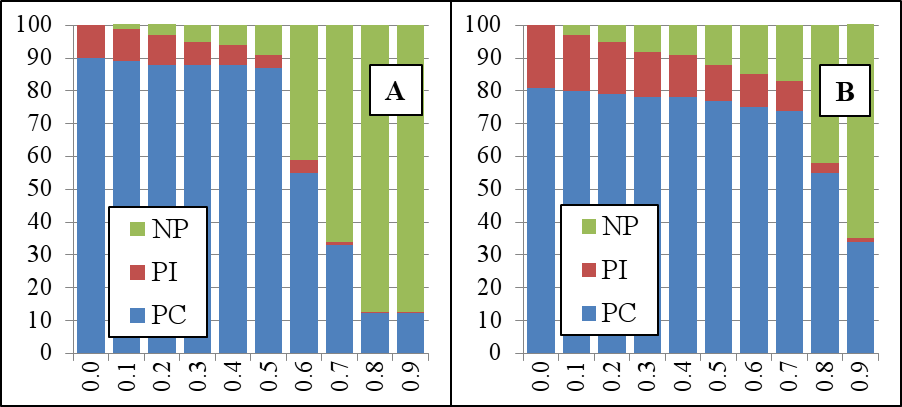
\includegraphics[width=100mm]{Figures/Fig67.png}
%\vspace{4pt}
\caption{\% of Products in each category for different values of $\tau$ on test data for $G_1$ in A)~Case-1 and	 B)~Case-2}
\label{fig:PC-2}
%\vspace{-14pt}
\end{figure}
\begin{figure}
\centering
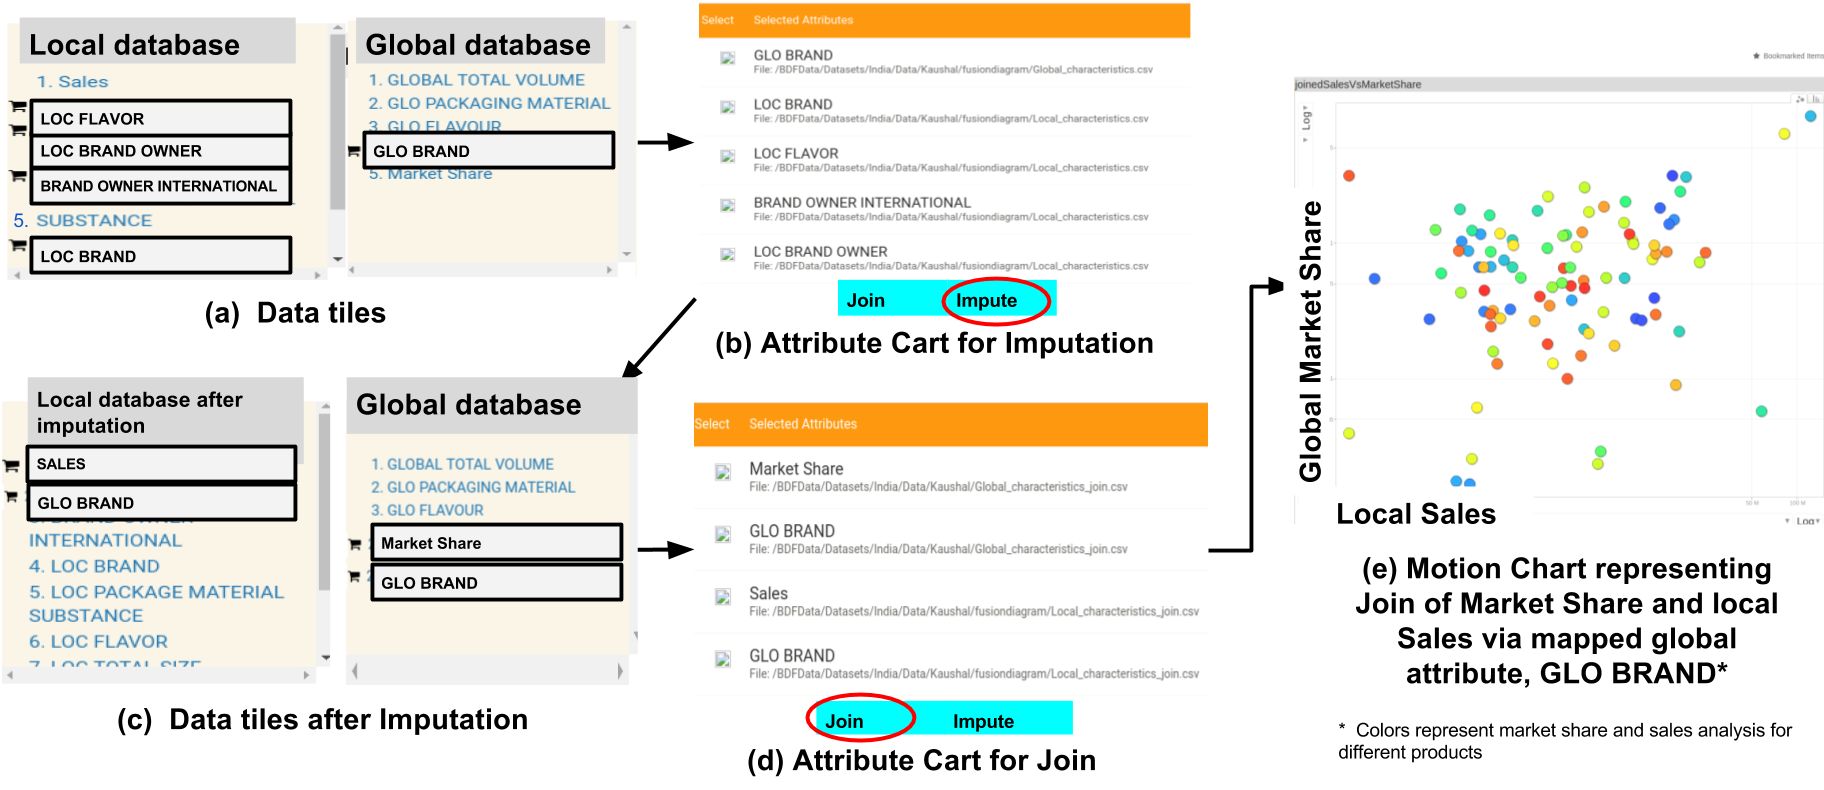
\includegraphics[width = 120mm]{Figures/EDBT_diagram3.png}
%\vspace{-8pt}
\caption{Figure showing aggregate analysis of global market share and local sales done using our platform. }
\label{fig:iFuse}
%\vspace{-12pt}
\end{figure}

% \begin{figure*}
% \centering
% \includegraphics[width=80mm]{Figures/iFuse}
% \vspace{1pt}
% \caption{jdd}
% \label{fig:iFuse}
% %\vspace{-16pt}
% \end{figure*}

\section{Conclusion}
\label{sec:conclusion}

This paper presents a matrix factorization based approach to text
outlier analysis. The approach is designed to adjust well to the
widely varying structures in different localities of the data, and
therefore provides more robust methods than competing models. The
approach has the potential to be applied to other domains with
similar structure, and as a specific example, we provide experiments
on market  basket data. We also presented extensive experimental
results, which illustrate the superiority of the approach.  
Our code can be downloaded from 
\url{https://github.com/ramkikannan/outliernmf} and 
tried with any text dataset. 

In this paper, we had a parallel implementation using the
Matlab's parallel computing toolbox to run in multicore environments.
In the future, we would like to explore a scalable implementation
of our algorithm. The solution is embarrassingly parallelizable,
and would like to experiment in web scale data. One of the potential
extension is incorporating temporal and spatial aspects into the model.
Such an extension, make the solution applicable to emerging 
applications such as topic detection and streaming data. 
%In the recent times,
%approximate matrix factorization techniques are explored by
%randomly sampling the input matrix. We can reduce the computation
%time for very large matrices using such sampling techniques. We would like
%to explore a sampling based solution for our model. 
We experimented
the solution primarily on text data and market basket data. In future
work, we will extend this broader approach to other domains such as
video data.



\section*{Acknowledgement} This work was supported by the National Natural Science Foundation of China under Contract 61472011.



{
\bibliographystyle{named}
\bibliography{egbib}
}

\end{document}
